\section{Metoda średniej ważonej ({\it importance sampling})}
%%%%%%%%%%%%%%%%
\begin{frame}{Metoda średniej ważonej}
	$f(x) = const.$ - w met. podstawowej - poj. punkt to wynik dokładny \\
    stąd: $f(x)$ - gładkie - liczba losowań - mała
    \\[8pt]
    Met. średniej ważonej - $g(x)$ - ciągła, $x \in [0, 1]$:
    \begin{enumerate}
    	\item $g(x) > 0, x \in [0, 1]$
        \item $\int_0^1 g(x) dx = 1$
        \item $\frac{f(x)}{g(x)}, x \in (0, 1)$ - znacznie gładsza niż $f(x)$
        \item $g(x)$ - dana prostym wzorem analitycznym
    \end{enumerate}
    
    \[
    	\left.
        	\begin{array}{ll}
        		\text{1, 2 - precyzyjne} \\
        		\text{3, 4 - rozmyte}
        	\end{array}
        \right\} 
        \text{warunki}
    \]
\end{frame}
%%%%%%%%%%%%%%%%
\begin{frame}{Metoda średniej ważonej - dygresja}
	\begin{block}{Dygresja - sugestia, co do dobrego $g(x)$}
		$X$ - zmienna losowa, \\
        $G(x)$ - dystrybuanta X; $G(x) = P(X < x)$
        \\[8pt]
        niech $G(x)$ - funkcja ściśle rosnąca: \[
        	P[\underbrace{G(x)}_\eta < \underbrace{G(x')}_{\eta'}] = P(x < x') = \underbrace{G(x')}_{\eta'}
        \]
        
        {\bf wniosek:} Jeżeli zmienna losowa $X$ ma ściśle rosnącą dystrybuantę $G(x)$, to $G(x)$ ma rozkład równomierny na $(0, 1)$
	\end{block}
\end{frame}
%%%%%%%%%%%%%%%%
\begin{frame}{Metoda średniej ważonej - dygresja}
	\begin{block}{Dygresja - sugestia, co do dobrego $g(x)$}
    	... stąd - sposób obliczania $I = \int_0^1 f(x) dx$:
        \begin{enumerate}
        	\item $g_1(x) > 0$ - 1-sza propozycja,
            \item dobór stałej - $g(x) = \alpha g_1(x); \alpha \int_0^1 g_1(x) dx = 1$
            \item analitycznie: $G(x) = \int_0^x g(x') dx'$
            \item losujemy z rozkładem równomiernym: $y_1 \in (0, 1), i = 1, ..., N$
            \item rozwiązujemy $G(x_i) = y_i \Rightarrow x_i, i = 1, ..., N$
            \item przybliżona wartość całki: $I \approx \frac{1}{N} \sum_{i=1}^N f(x_i)$
        \end{enumerate}
	\end{block}
\end{frame}
%%%%%%%%%%%%%%%%
\begin{frame}{Metoda średniej ważonej - dygresja}
	\begin{block}{Dygresja - sugestia, co do dobrego $g(x)$}
    	\centering 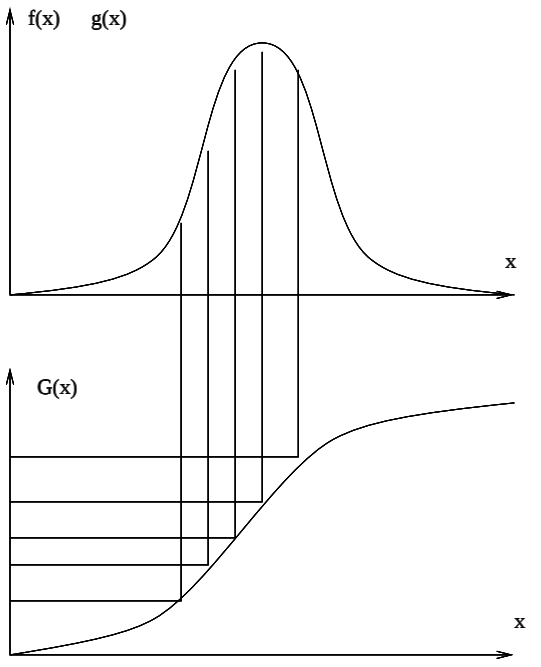
\includegraphics[width=.4\linewidth]{img/15/15_2_dobre_gx}
	\end{block}
\end{frame}